% vim:set spell tw=79:

\documentclass[beamer]{uibk}
\title{Exploitation Techniques and Mitigations}
\subtitle{Dark Arts of Computer Science}
\author{Alex Hirsch \and Patrick Ober}
\date{2016-01-15}

\usepackage{multicol}
\newminted{nasm}{fontsize=\scriptsize,frame=leftline,framesep=2mm,linenos}

\AtBeginSection[] {
    \begin{frame}{Outline}
        \begin{multicols}{2}
            \tableofcontents[currentsection]
        \end{multicols}
    \end{frame}
}

\begin{document}

\maketitle

\begin{frame}{Outline}
    \begin{multicols}{2}
        \tableofcontents
    \end{multicols}
\end{frame}

\begin{frame}{Acknowledgement}
    \begin{columns}
        \begin{column}{0.5\textwidth}
            We reuse a lot from MBE, a university course about modern binary
            exploitation at Rensselaer Polytechnic Institute (2015), because
            \dots

            \begin{description}
                \item[of them:] They did a great job
                \item[of you:] You will see familiar material
                \item[of us:] We are lazy
            \end{description}

            Check them out:\\
            \url{http://rpis.ec/}\\
            \url{https://github.com/RPISEC/MBE}
        \end{column}
        \begin{column}{0.5\textwidth}
            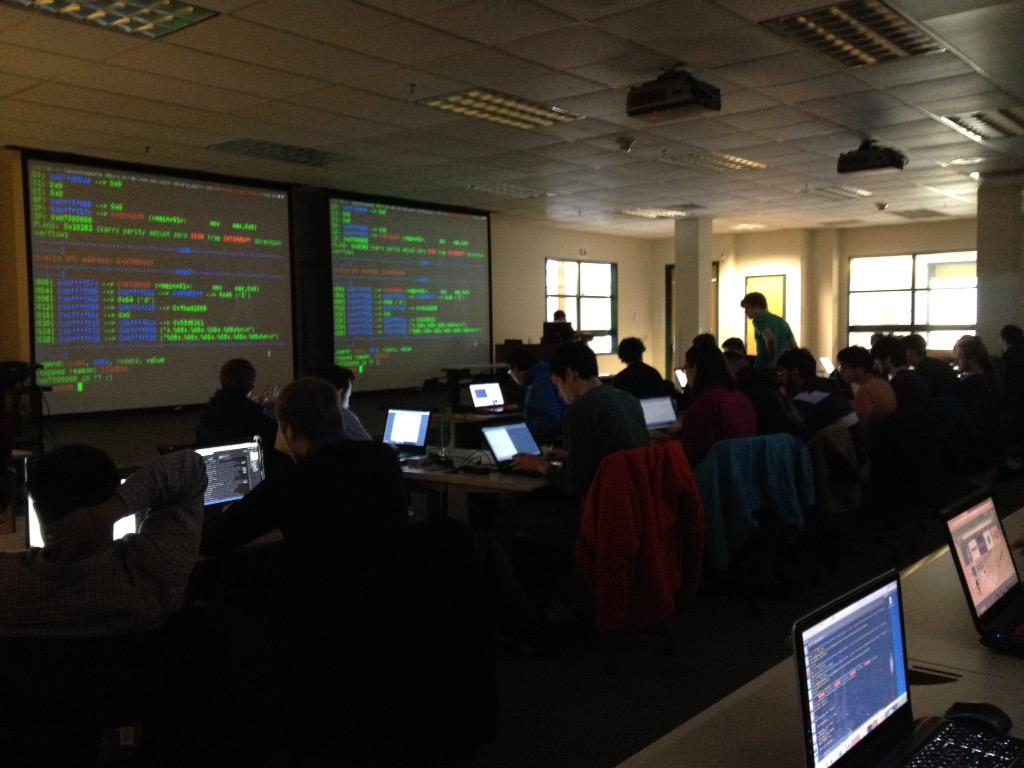
\includegraphics[height=0.7\textheight]{ripsec}
        \end{column}
    \end{columns}
\end{frame}

\section{Platform x86}

\begin{frame}{Why x86?}
    \begin{itemize}
        \item It's simpler, yet not overly simplified
        \item People call it \emph{more academic} \quad *sigh*
        \item Most techniques can be translated easily
        \item Most material covers x86
    \end{itemize}
    \bigskip
    Demonstrations: Ubuntu 14.04 LTS x86 inside VirtualBox
\end{frame}

\begin{frame}{Registers}
    \begin{center}
        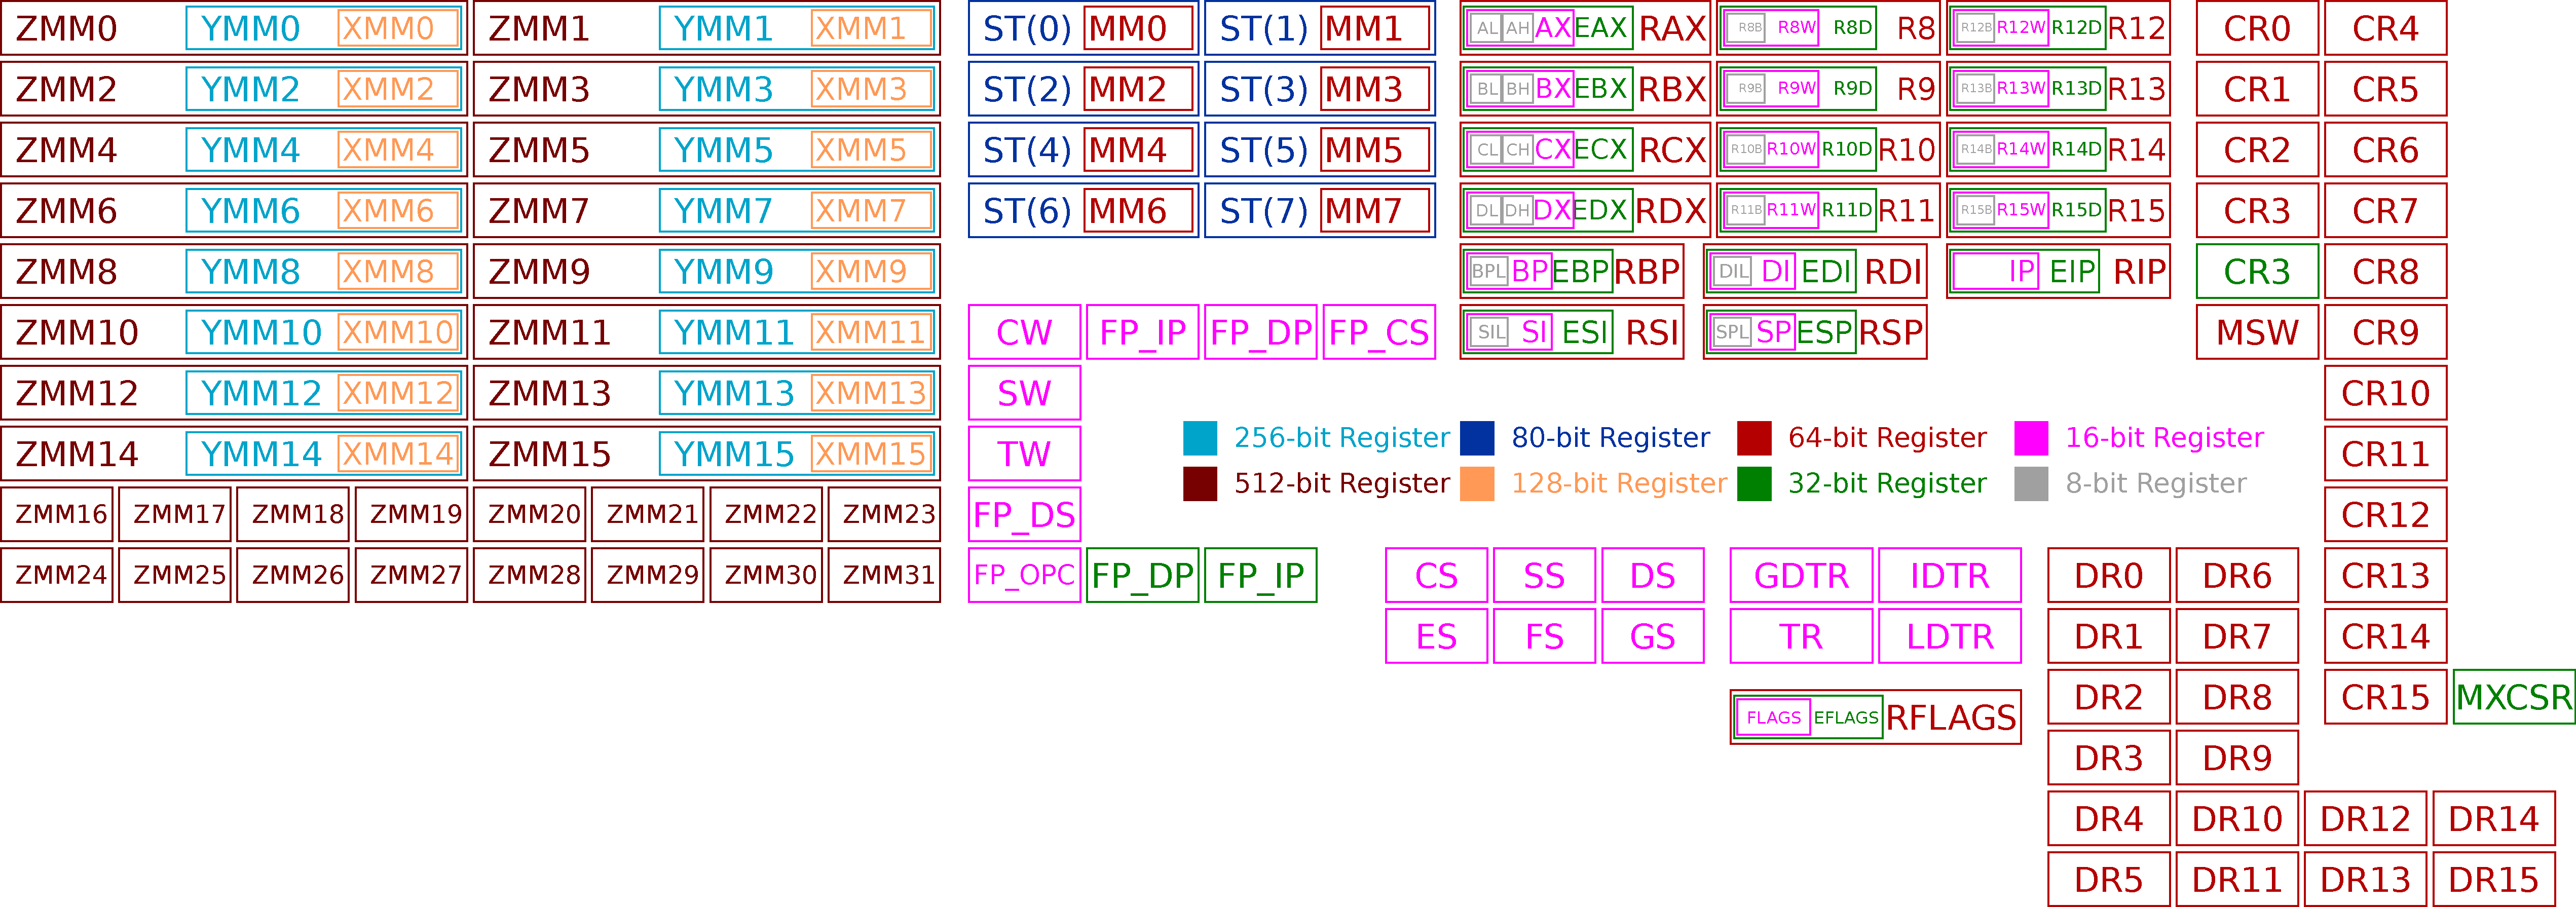
\includegraphics[width=\textwidth]{x86_registers}
    \end{center}
    \sidenote{- Wikipedia}
\end{frame}

\begin{frame}{Registers}
    \begin{columns}
        \begin{column}{0.45\textwidth}
            \begin{description}
                \item[\texttt{EAX}] Accumulator Register
                \item[\texttt{EBX}] Base Register
                \item[\texttt{ECX}] Counter Register
                \item[\texttt{EDX}] Data Register
                \item[\texttt{ESI}] Source Index
                \item[\texttt{EDI}] Destination Index
                \item[\texttt{EBP}] Base Pointer
                \item[\texttt{ESP}] Stack Pointer
            \end{description}
        \end{column}
        \begin{column}{0.55\textwidth}
                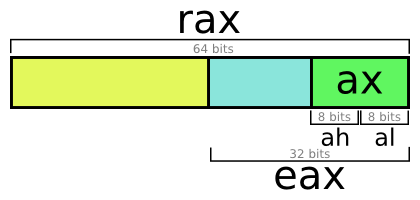
\includegraphics[width=\textwidth]{single_register}
        \end{column}
    \end{columns}
    \sidenote{- \url{http://www.swansontec.com/sregisters.html} /
    \url{http://nullprogram.com/}}
\end{frame}

\begin{frame}{Memory Management}
    \begin{columns}
        \begin{column}{0.5\textwidth}
            \begin{itemize}
                \item Kernel manages physical memory\\
                    through \textbf{memory management unit} (hardware)
                \medskip
                \item Process sees only \textbf{virtual} memory
                \medskip
                \item \SI{4}{\kibi\byte} typical page size
                \medskip
                \item Addresses can be decomposed (page pointer + offset):\\
                    \smallskip
                    $\mathtt{0xA1B2C3D4} \to \texttt{0xA1B2C000} + \mathtt{0x3D4}$
            \end{itemize}
        \end{column}
        \begin{column}{0.5\textwidth}
            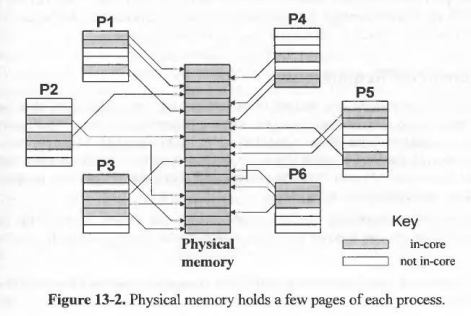
\includegraphics[height=0.65\textheight]{pages}
        \end{column}
    \end{columns}
    \sidenote{- Unix Internals by Uresh Vahalia}
\end{frame}

\begin{frame}{Process' Memory}
    \begin{columns}
        \begin{column}{0.5\textwidth}
            \begin{center}
                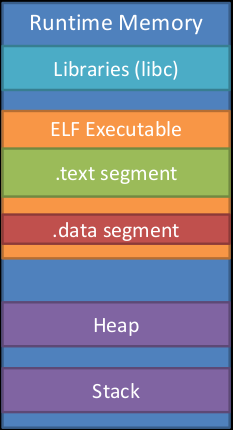
\includegraphics[height=0.8\textheight]{mem_layout}
            \end{center}
        \end{column}
        \begin{column}{0.5\textwidth}
            You may already know some of this.
            \bigskip

            What we'll see today:
            \begin{itemize}
                \item Pages have permissions \texttt{rwx} (DEP)
                \item Layout not always the same (ASLR)
                \item Stack layout
                \item Lots of pointers
            \end{itemize}
        \end{column}
    \end{columns}
\end{frame}

\begin{frame}[fragile]{System Call \& Protection Rings}
    \begin{columns}
        \begin{column}{0.55\textwidth}
            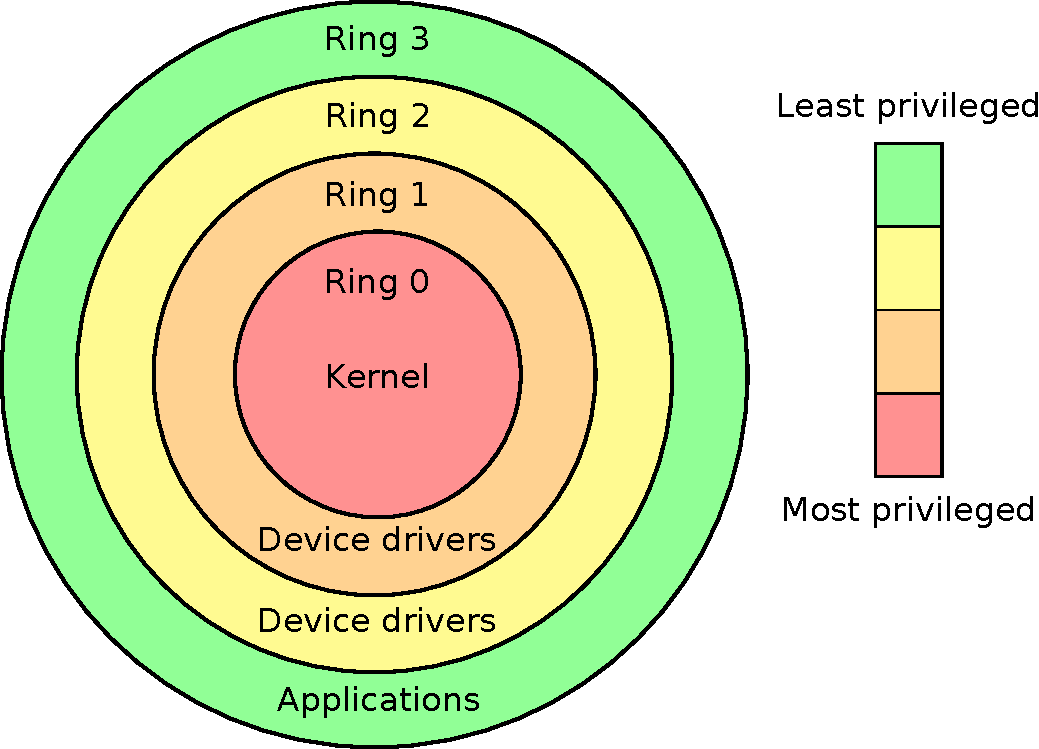
\includegraphics[width=\textwidth]{x86_rings}
        \end{column}
        \begin{column}{0.45\textwidth}
            Your CPU can switch from a more privileged state to a less
            privileged one
            \bigskip

            Kernel does not run always, process cannot do everything (enforced
            by hardware)
            \bigskip

            Process uses \emph{System Calls} to notify the kernel to take over
            (context switch)
            \medskip

            \begin{nasmcode*}{autogobble,linenos=false}
                int   0x80   ; old, but still works
                call  write  ; new, sysenter via VDSO
            \end{nasmcode*}
        \end{column}
    \end{columns}
    \sidenote{- Wikipedia}
\end{frame}

\begin{frame}{System Calls}
    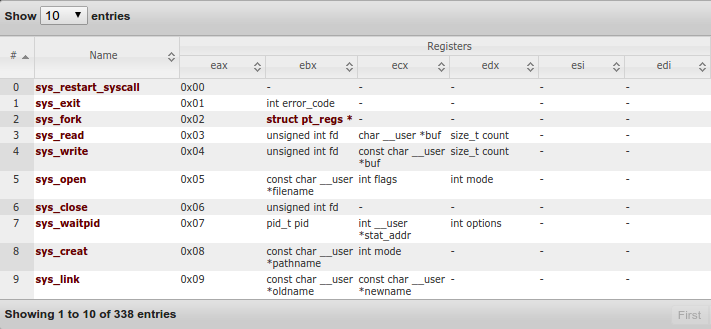
\includegraphics[width=\textwidth]{systemcalls}
    \sidenote{- \url{http://syscalls.kernelgrok.com/}}
\end{frame}

\begin{frame}{Endianness}
    \begin{columns}
        \begin{column}{0.5\textwidth}
            \begin{center}
                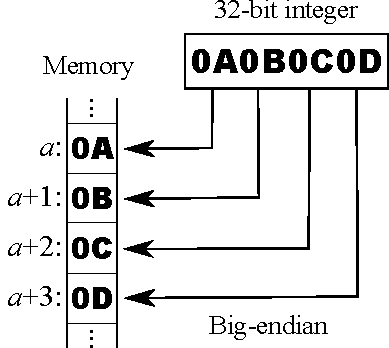
\includegraphics[width=0.8\textwidth]{big_endian}
            \end{center}
        \end{column}
        \begin{column}{0.5\textwidth}
            \begin{center}
                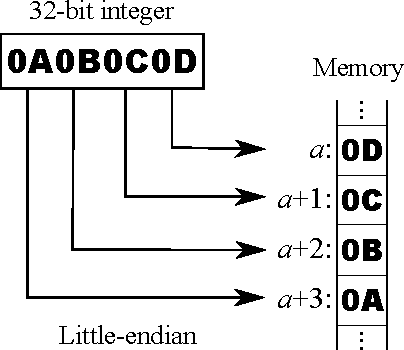
\includegraphics[width=0.8\textwidth]{little_endian}
            \end{center}
        \end{column}
    \end{columns}
    \sidenote{- Wikipedia}
\end{frame}

\begin{frame}{Calling Convention}
    \begin{columns}
        \begin{column}{0.5\textwidth}
            Defines:
            \begin{itemize}
                \item Where to place arguments
                \item Where to place return value
                \item Where to place return address
                \item Who prepares the stack
                \item Who cleans up\\
                    (caller or callee)
            \end{itemize}
            \pause
            Depends on:
            \begin{itemize}
                \item Your platform
                \item Your toolchain (language)
                \item Your settings (compiler flags)
            \end{itemize}
        \end{column}
        \pause
        \begin{column}{0.5\textwidth}
            \textbf{C Declaration (cdecl):}
            \begin{itemize}
                \item Arguments on stack (reverse order)\\
                    stack aligned to \SI{16}{\byte} boundary
                \item Return via register (\texttt{EAX} / \texttt{ST0})
                \item On stack:\\
                    old instruction pointer (\texttt{IP})\\
                    old base pointer (\texttt{BP})
                \item Caller does the cleanup
            \end{itemize}
        \end{column}
    \end{columns}
\end{frame}

\begin{frame}{Main Assumption}
   \begin{center}
       \huge The target binary and libraries are known.
   \end{center}
\end{frame}

\section{Exploit printf}

\begin{frame}[fragile]{Death by \texttt{printf}}
    \begin{columns}
        \begin{column}{0.5\textwidth}
            \cfile[xleftmargin=0.8cm,firstline=4]{../format_string/main.c}
        \end{column}
        \begin{column}{0.5\textwidth}
            \pause
            \begin{pre*}{autogobble}
                ~> echo foobar | ./main
                You entered:
                foobar
            \end{pre*}
            \bigskip\pause
            \begin{pre*}{autogobble}
                ~> echo AAAABBBB | ./main
                correct
            \end{pre*}
            \bigskip\pause
            \begin{pre*} {autogobble}
                ~> echo '%08x' | ./main
                You entered:
                bfd98ed4
            \end{pre*}
            \medskip
            Oh look, a pointer, this may come in handy
        \end{column}
    \end{columns}
\end{frame}

\begin{frame}{Death by \texttt{printf}}
    \begin{center}
        \huge Demonstration
    \end{center}
\end{frame}

\begin{frame}{Death by \texttt{printf}}
    \begin{itemize}
        \item Even functions which look very simple / basic can be exploited
        \bigskip
        \item RTFM
        \bigskip
        \pause
        \item But it gets better \dots
    \end{itemize}
\end{frame}

\begin{frame}{\texttt{printf} Oriented Programming}
    \begin{center}
        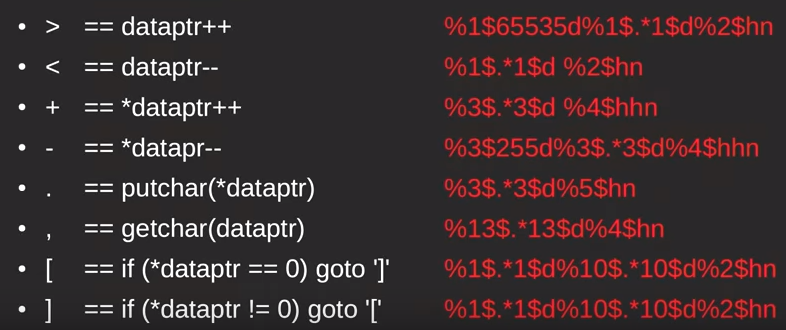
\includegraphics[width=0.8\textwidth]{printbf}
    \end{center}

    Brainfuck to \texttt{printf} format string compiler:\\
    \url{http://github.com/HexHive/printbf}
    \sidenote{- New memory corruption attacks {[}32c3{]}}
\end{frame}

\section{Buffer Overflow}

\begin{frame}[fragile]{Variants}
    \begin{columns}
        \begin{column}{0.5\textwidth}
            Static Memory Corruption
        \end{column}
        \begin{column}{0.5\textwidth}
            \begin{ccode*}{autogobble,linenos=false}
                void foo(void) {
                    static char buffer[64];
                    /* ... */
                }
            \end{ccode*}
        \end{column}
    \end{columns}
    \medskip
    \pause
    \begin{columns}
        \begin{column}{0.5\textwidth}
            Dynamic Memory (Heap) Corruption
        \end{column}
        \begin{column}{0.5\textwidth}
            \begin{ccode*}{autogobble,linenos=false}
                void foo(void) {
                    char *buffer = (char *) malloc(64);
                    /* ... */
                    free(buffer);
                }
            \end{ccode*}
        \end{column}
    \end{columns}
    \medskip
    \pause
    \begin{columns}
        \begin{column}{0.5\textwidth}
            Stack Smashing
        \end{column}
        \begin{column}{0.5\textwidth}
            \begin{ccode*}{autogobble,linenos=false}
                void foo(void) {
                    char buffer[64];
                    /* ... */
                }
            \end{ccode*}
        \end{column}
    \end{columns}
\end{frame}

\begin{frame}{Smashing the Stack}
    \begin{columns}
        \begin{column}{0.5\textwidth}
            \begin{center}
                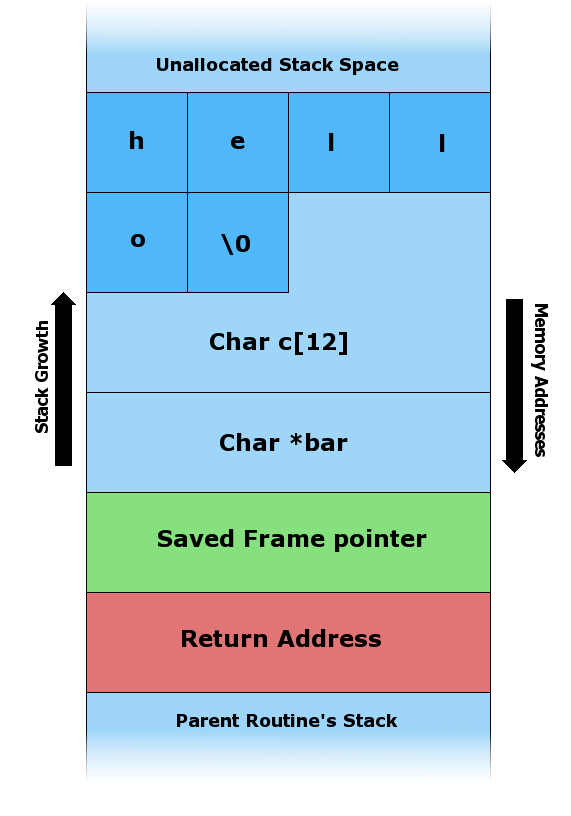
\includegraphics[width=0.75\textwidth]{stack_smash}
            \end{center}
        \end{column}
        \begin{column}{0.5\textwidth}
            \begin{itemize}
                \item Here, you write from top to bottom \bigskip
                \item You'll first overwrite local variables (\texttt{bar}) \bigskip
                \item Followed by arguments \bigskip
                \item Your \textbf{saved return address} \bigskip
                \item The next frame
            \end{itemize}
        \end{column}
    \end{columns}
    \sidenote{- Wikipedia}
\end{frame}

\begin{frame}{Return to a Different Function}
    \begin{center}
        \huge Demonstration
    \end{center}
\end{frame}

\section{Shell Code}

\begin{frame}{Idea}
    \begin{itemize}
        \item Supply executable binary code via buffer
        \medskip
        \item Rewrite return address to point into buffer
        \medskip
        \item Binary code opens a shell upon execution
    \end{itemize}
\end{frame}

\begin{frame}[fragile]{Example}
    \begin{columns}
        \begin{column}{0.55\textwidth}
            \begin{pre*}{autogobble,xleftmargin=1em}
                > cat shellcode.asm
            \end{pre*}
            \begin{nasmcode*}{autogobble,xleftmargin=1em}
                xor     eax, eax    ;Clearing eax register
                push    eax         ;Pushing NULL bytes
                push    0x68732f2f  ;Pushing //sh
                push    0x6e69622f  ;Pushing /bin
                mov     ebx, esp    ;ebx now has address of /bin//sh
                push    eax         ;Pushing NULL byte
                mov     edx, esp    ;edx now has address of NULL byte
                push    ebx         ;Pushing address of /bin//sh
                mov     ecx, esp    ;ecx now has address of address
                                    ;of /bin//sh byte
                mov     al, 11      ;syscall number of execve is 11
                int     0x80        ;Make the system call
            \end{nasmcode*}
        \end{column}
        \begin{column}{0.45\textwidth}
            \begin{pre*}{autogobble}
                > nasm -f elf shellcode.asm
                > objdump -d -M intel shellcode.o
                00000000 <.text>:
                   0:  31 c0                  xor    eax,eax
                   2:  50                     push   eax
                   3:  68 2f 2f 73 68         push   0x68732f2f
                   8:  68 2f 62 69 6e         push   0x6e69622f
                   d:  89 e3                  mov    ebx,esp
                   f:  50                     push   eax
                  10:  89 e2                  mov    edx,esp
                  12:  53                     push   ebx
                  13:  89 e1                  mov    ecx,esp
                  15:  b0 0b                  mov    al,0xb
                  17:  cd 80                  int    0x80
            \end{pre*}
        \end{column}
    \end{columns}
    \bigskip

    Result:
    \begin{pre*}{autogobble}
        \x31\xc0\x50\x68\x2f\x2f\x73\x68\x68\x2f\x62\x69\x6e\x89\xe3\x50\x89\xe2\x53\x89\xe1\xb0\x0b\xcd\x80
    \end{pre*}

    \sidenote{- \url{https://dhavalkapil.com/blogs/Shellcode-Injection/}}
\end{frame}

\begin{frame}{Inject Shell Code}
    \begin{center}
        \huge Demonstration
    \end{center}
\end{frame}

\begin{frame}[fragile]{Putting it together}
    \begin{itemize}
        \item Starting position of the stack varies because of environment
            variables\\
            \medskip
            $\implies$ prepend shellcode with \textit{NOP Sled} to improve our
            odds
        \bigskip
        \item Return address will be located after \texttt{buf}\\
            \medskip
            $\implies$ append \texttt{'A'}s to our shellcode until we reach the
            return address
        \bigskip
        \item Aim for the center of the \textit{NOP Sled}\\
            \medskip
            $\mathit{target} = \frac{\mathrm{length}(\text{NOP Sled})}{2}\ +\ \mathrm{length}(\text{shellcode})\ +\ \#(\texttt{A})\ +\ \texttt{\&RET}$
   \end{itemize}
   \begin{center}
       \usetikzlibrary{arrows.meta}
\usetikzlibrary{shapes.multipart}

\tikzstyle{block} = [
	draw,
	align=center,
	rectangle,
]

\tikzstyle{block split} = [
	block,
	rectangle split,
	rectangle split horizontal,
	rectangle split part align=base,
]

\tikzstyle{ptr}=[
	-{Latex[length=2.7mm]}
]

\begin{tikzpicture}

\node[block split] (payload) {
	\nodepart{one}    \texttt{NOP} Sled
	\nodepart{two}    Shell Code
	\nodepart{three}  AAA\dots AAA
	\nodepart{four}   \textit{target}
};

\draw [ptr] (payload.four south) -- +(0,-0.5) -| (payload.one south);

\end{tikzpicture}

   \end{center}
\end{frame}

\section{Data Execution Prevention (DEP)}

\begin{frame}{Data Execution Prevention}
    \begin{columns}
        \begin{column}{0.5\textwidth}
            \begin{center}
                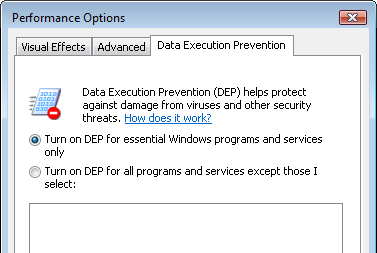
\includegraphics[width=1.1\textwidth]{dep_windows}
            \end{center}
            \medskip

            Using Windows? Have a look at \texttt{VMMap.exe} from Sysinternals Suite
        \end{column}
        \begin{column}{0.5\textwidth}
            \begin{itemize}
                \item Also known as \textbf{write XOR execute} (\texttt{w\^{}x})
                \medskip
                \item Sometimes called \textbf{page protection}
                \bigskip
                \item Typically enforced by hardware
                \medskip
                \item \texttt{rwx} permissions per memory page
                \medskip
                \item \texttt{segfault} is triggered upon violation
            \end{itemize}
        \end{column}
    \end{columns}
\end{frame}

\begin{frame}{Data Execution Prevention}
    \begin{block}{Famous Quote}
        If your program simply segfaulted, consider yourself lucky.
    \end{block}
\end{frame}

\begin{frame}{Data Execution Prevention}
    \begin{itemize}
        \item We cannot execute supplied code anymore =(
        \item What now?
        \bigskip
        \pause
        \item Take control!
    \end{itemize}
\end{frame}

\section{Return Oriented Programming (ROP)}

\begin{frame}{Idea}
    \begin{itemize}
        \item Target may not have a \texttt{gimme\_shell\_plz} function.
        \bigskip
        \pause
        \item Create such a function by combining parts (\textbf{gadgets}) of
            available functions.
        \bigskip
        \item x86 allows us to jump to \emph{any} location (even between
            instructions)
    \end{itemize}
\end{frame}

\begin{frame}[fragile]{Gadgets}
    \begin{columns}
        \begin{column}{0.6\textwidth}
            \begin{pre*}{autogobble}
                > objdump -d /lib/i386-linux-gnu/libc.so.6 | grep -B5 ret
                  ...
                18f59:       8b 54 24 04             mov    0x4(%esp),%edx
                18f5d:       83 c4 20                add    $0x20,%esp
                18f60:       5e                      pop    %esi
                18f61:       5f                      pop    %edi
                18f62:       5d                      pop    %ebp
                18f63:       c3                      ret
                  ...
                192d4:       8b 54 24 2c             mov    0x2c(%esp),%edx
                192d8:       e8 23 fc ff ff          call   18f00 <__floatdidf+0x30>
                192dd:       8b 44 24 18             mov    0x18(%esp),%eax
                192e1:       8b 54 24 1c             mov    0x1c(%esp),%edx
                192e5:       83 c4 24                add    $0x24,%esp
                192e8:       c3                      ret
                  ...
            \end{pre*}
        \end{column}
        \begin{column}{0.4\textwidth}
            \begin{itemize}
                \item \textbf{Definition:} Sequence of instructions ending with
                    \texttt{RET}
                \bigskip
                \item Target addresses are provided through the buffer and used
                    one by one on \texttt{ret}
                \bigskip
                \item We can also use library functions (\textit{ret2libc})
            \end{itemize}
        \end{column}
    \end{columns}
    \sidenote{- \url{https://crypto.stanford.edu/~blynn/rop/}}
\end{frame}

\begin{frame}{Return2libc}
    \begin{center}
        \huge Demonstration
    \end{center}
\end{frame}

\section{Address Space Layout Randomization (ASLR)}

\begin{frame}{Idea}
    \begin{itemize}
        \item Randomize the location of (some) segments every time the program
            is run
        \bigskip
        \pause
        \item Return oriented programming cannot be used reliably anymore
    \end{itemize}
\end{frame}

\begin{frame}[fragile]{\texttt{/proc/self/maps}}
    \begin{pre*}{autogobble}
        ~> cat /proc/self/maps
        08048000-08054000 r-xp 00000000 08:01 131085     /bin/cat
        08054000-08055000 r--p 0000b000 08:01 131085     /bin/cat
        08055000-08056000 rw-p 0000c000 08:01 131085     /bin/cat
        08905000-08926000 rw-p 00000000 00:00 0          [heap]
        b758d000-b7741000 r-xp 00000000 08:01 917531     /lib/i386-linux-gnu/libc-2.21.so
        b7752000-b7753000 r-xp 00000000 00:00 0          [vdso]
        bfb26000-bfb47000 rw-p 00000000 00:00 0          [stack]
    \end{pre*}
    \bigskip
    some lines have been omitted
\end{frame}
\begin{frame}[fragile]{\texttt{/proc/self/maps}}
    \begin{pre*}{autogobble}
        ~> cat /proc/self/maps
        08048000-08054000 r-xp 00000000 08:01 131085     /bin/cat
        08054000-08055000 r--p 0000b000 08:01 131085     /bin/cat
        08055000-08056000 rw-p 0000c000 08:01 131085     /bin/cat
        0954e000-0956f000 rw-p 00000000 00:00 0          [heap]
        b7595000-b7749000 r-xp 00000000 08:01 917531     /lib/i386-linux-gnu/libc-2.21.so
        b775a000-b775b000 r-xp 00000000 00:00 0          [vdso]
        bfbc9000-bfbea000 rw-p 00000000 00:00 0          [stack]
    \end{pre*}
    \bigskip
    some lines have been omitted
\end{frame}
\begin{frame}[fragile]{\texttt{/proc/self/maps}}
    \begin{pre*}{autogobble}
        ~> cat /proc/self/maps
        08048000-08054000 r-xp 00000000 08:01 131085     /bin/cat
        08054000-08055000 r--p 0000b000 08:01 131085     /bin/cat
        08055000-08056000 rw-p 0000c000 08:01 131085     /bin/cat
        0913e000-0915f000 rw-p 00000000 00:00 0          [heap]
        b75cc000-b7780000 r-xp 00000000 08:01 917531     /lib/i386-linux-gnu/libc-2.21.so
        b7791000-b7792000 r-xp 00000000 00:00 0          [vdso]
        bf8f8000-bf919000 rw-p 00000000 00:00 0          [stack]
    \end{pre*}
    \bigskip
    some lines have been omitted
\end{frame}

\begin{frame}{Breaking ASLR}
    \begin{itemize}
        \item \texttt{.text} segment starts at \texttt{0x00400000} if not
            compiled with PIE (position independent executable)
        \medskip
        \pause
        \item \textbf{Info leak:} If we manage to get pointer from the program
            we can calculate the ASLR offset, Remember the first example with
            \texttt{printf}
        \medskip
        \item \textbf{Brute Force:} Guessing may be a viable option on
            \SI{32}{\bit}
    \end{itemize}
\end{frame}

\begin{frame}{Info Leak Example}
    Lets say you managed to leak a pointer (\texttt{0xb7e72280}) and you know
    that this one usually points to \texttt{printf}.
    \bigskip

    Look how far away \texttt{system} is from \texttt{printf}, in the standard
    library. It's \texttt{0xD0F0} bytes.
    \bigskip

    We now know that \texttt{system} is at:
    \[ \mathtt{0xb7e72280} - \mathtt{0xD0F0} = \mathtt{0xb7e65190} \]
\end{frame}

\section{Stack Cookies (Canary)}

\begin{frame}{Idea}
    Put something between buffer and return address, which guards the return
    address
    \bigskip
    \pause
    \begin{description}
        \item[Terminator canaries:] Render \textbf{string operations}
            useless by placing a terminator (\texttt{null},
            \texttt{\textbackslash r}, \texttt{\textbackslash n},
            \texttt{-1}) before return address
        \medskip
        \item [Random canaries:] Generate a random value, store somewhere
            \textit{safe}, place on the stack and check before each return
            whether this value is still the same
        \medskip
        \item [Random XOR canaries:] Same as above but scrambled to mitigate
            \textit{read-from-stack}
    \end{description}
\end{frame}

\begin{frame}[fragile]{A look at GCC}
    \sidenote{- \url{http://0x90.at/post/gdb-stack-script}}
    \begin{columns}
        \begin{column}{0.5\textwidth}
            \cfile[xleftmargin=0.8cm]{../canary/main.c}
            \begin{pre*}{autogobble,xleftmargin=0.8cm}
                > gcc --version
                gcc (Ubuntu 5.2.1-22ubuntu2) 5.2.1 20151010
                  ...
                > gcc -g -o main main.c
            \end{pre*}
        \end{column}
        \pause
        \begin{column}{0.5\textwidth}
            \begin{pre*}{autogobble}
                > gdb ./main
                AAAAAAA
                  ...
                Breakpoint 1, 0x0000000000400671 in fun ()
                (gdb) show-stack
                Stack
                ------------------------
                0xbffff550: 0x00000003             <-- esp
                0xbffff554: 0x41414141             <-- buf
                0xbffff558: 0x0a414141
                0xbffff55c: 0x17981f00             <-- canary
                       (padding)
                       (padding)
                0xbffff568: 0xbffff578 (Saved RBP) <-- ebp
                0xbffff56c: 0x0804852a (Saved RIP)
                ------------------------
            \end{pre*}
        \end{column}
    \end{columns}
\end{frame}

\begin{frame}{Breaking the canary}
    \begin{columns}
        \begin{column}{0.4\textwidth}
            \begin{center}
                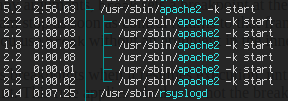
\includegraphics[width=1.1\textwidth]{workers.png}
            \end{center}
        \end{column}
        \pause
        \begin{column}{0.6\textwidth}
            \begin{itemize}
                \item Server \textbf{forks} multiple times to create workers
                \item Memory is handled copy-on-write\\
                    $\implies$ all workers share the same canary
                \item Server respawns workers if they die
                \item $\implies$ infinite guesses
            \end{itemize}
        \end{column}
    \end{columns}
    \bigskip
    \pause
    Most of the time you can write byte by byte and the first byte is $0$:
    \begin{align*}
        \implies 2^8 \times 3 & = 768  & \text{ guesses at most \SI{32}{\bit}}\\
        \implies 2^8 \times 7 & = 1792 & \text{ guesses at most \SI{64}{\bit}}
    \end{align*}
\end{frame}

\section{Heap Corruption}

\begin{frame}{Heap vs. Stack}
    \begin{itemize}
        \item Managed by the programmer through \texttt{malloc} /
            \texttt{calloc} / \texttt{recalloc} / \texttt{free}
        \medskip
        \item Mainly used for structs (objects), big buffers, persistent data
        \medskip
        \item \textbf{non-linear} structure
        \medskip
        \item Many different implementations (dlmalloc, ptmalloc, \dots)\\
            some applications come with their own implementation
        \medskip
        \item Details depend \emph{heavily} on implementation
    \end{itemize}
\end{frame}

\begin{frame}{Overflow}
    \begin{columns}
        \begin{column}{0.5\textwidth}
            \begin{center}
                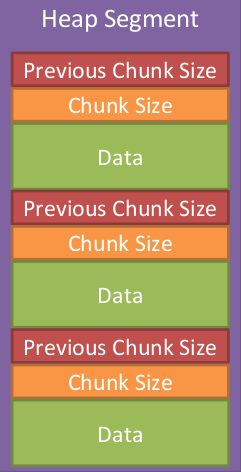
\includegraphics[height=0.9\textheight]{heap_segment}
            \end{center}
        \end{column}
        \begin{column}{0.5\textwidth}
            \begin{center}
                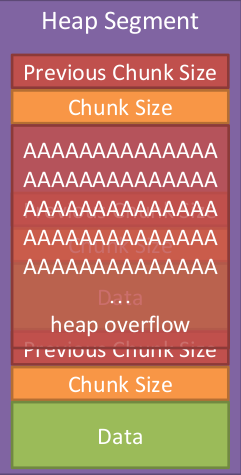
\includegraphics[height=0.9\textheight]{heap_overflow}
            \end{center}
        \end{column}
    \end{columns}
\end{frame}

\begin{frame}{Attack Surface}
    \begin{itemize}
        \item Anything that handles the now corrupted data can be viewed as
            additional attack surface
        \medskip
        \pause
        \item Structs commonly contain function pointers which can be
            overwritten
        \bigskip
        \pause
        \item \textbf{Use After Free:} Pointer gets still used somewhere after
            \texttt{free}, pointer target is now attack surface, extremely
            common complex programs (browsers)
        \medskip
        \item \textbf{Heap Spraying:} Fill heap with exploitable code, viable
            on \SI{32}{\bit}, not so on \SI{64}{\bit} (\textasciitilde
            \SI{18446744}{\tera\byte})
    \end{itemize}
\end{frame}

\section{Control Flow Integrity (CFI)}

\begin{frame}{Control Flow Graph}
    \begin{center}
        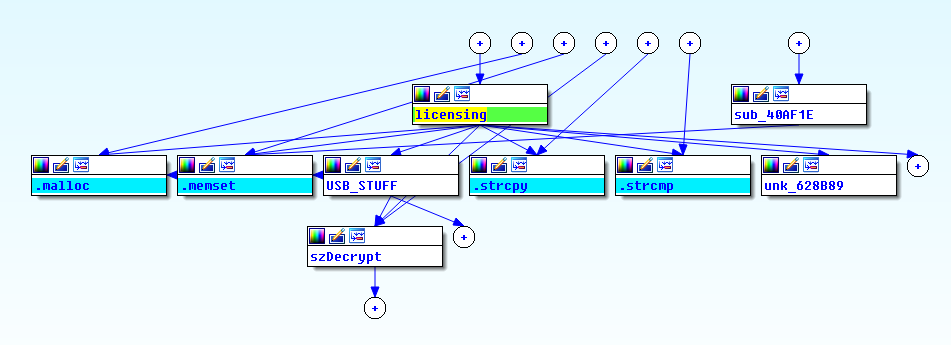
\includegraphics[width=\textwidth]{gfx/unraid_part_graph.png}
    \end{center}
    \sidenote{- unRAID emhttp inside IDA}
\end{frame}

\begin{frame}{Control Flow Integrity}
    \begin{itemize}
        \item Construct a set for each function $f$ containing all functions
            where $f$ gets called
        \bigskip
        \item Check actual return destination against this set
        \medskip
        \item Abort if destination is not an element of the specific set
    \end{itemize}
\end{frame}

\begin{frame}{Control Flow Bending}
    \begin{center}
        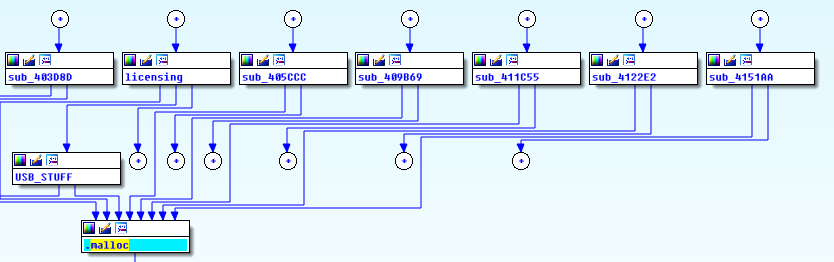
\includegraphics[width=\textwidth]{gfx/unraid_part_graph_malloc.png}
    \end{center}
    \sidenote{- unRAID emhttp inside IDA}
\end{frame}

\begin{frame}{Control Flow Bending}
    \begin{itemize}
        \item Control flow graph is heavily connected via common functions,
                like \texttt{printf}, \texttt{malloc}, \texttt{memcpy}, \dots
        \medskip
        \item Such functions make it easy to transition from the attackers
            entry point to his target location (\texttt{system})
        \medskip
        \item Transitions from function to function are valid (with respect to
            Control Flow Integrity)
        \medskip
        \item $\implies$ whole path is malicious
    \end{itemize}
\end{frame}

\begin{frame}{Stack Integrity}
    \begin{itemize}
        \item Place return address on a \textit{shadow stack}
        \medskip
        \item \textit{shadow stack} protected by hardware
        \medskip
        \item $\implies$ Function can only return to its current caller
        \medskip
        \item $\implies$ Cannot bend control flow anymore
    \end{itemize}
\end{frame}

\begin{frame}{Breaking Stack Integrity}
    \begin{itemize}
        \item Idea: If the program contains a Turing complete
            \textbf{interpreter}, we can just use it to execute our malicious
            code.
        \bigskip
        \pause
        \item \texttt{printf} is such an interpreter
    \end{itemize}
\end{frame}

\begin{frame}{Outlook}
    \begin{center}
        Code Pointer Integrity \quad (Volodymyr Kuznetsov \textit{et al.})
    \end{center}
\end{frame}

% \section{Fuzzing}

\section{Polymorphic Code}

\begin{frame}{Polymorphism}
    \begin{center}
        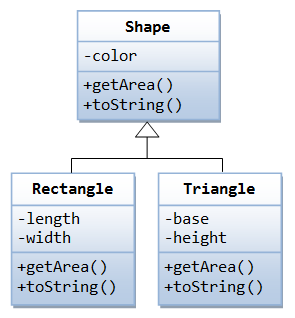
\includegraphics[height=0.7\textheight]{polymorphism}
    \end{center}
    \sidenote{\url{- ntu.edu.sg}}
\end{frame}

\begin{frame}{\st{Polymorphism} Polymorphic Code}
    \begin{itemize}
        \item code which \emph{evolves} during runtime
        \item often malicious code, but also used in DRM
        \item makes use of encryption
        \medskip
        \pause
        \item makes static analysis hard, you basically need to reverse
            engineer the system,\\
            running it may not reveal all parts or be straight up lethal!
    \end{itemize}
\end{frame}

\begin{frame}{\st{Polymorphism} Polymorphic Code}
    \begin{itemize}
        \item malicious parts sometimes only triggered when special conditions
            are met (time, platform, events, \dots)
        \medskip
        \pause
        \item \textbf{metamorphic engines} are used to generated new code;\\
            little documentation / public knowledge;\\
            some even see it as taboo
        \medskip
        \pause
        \item have a look at \url{http://z0mbie.daemonlab.org/}\\
            and \url{http://vxheaven.org/lib/vmd01.html}
    \end{itemize}
\end{frame}

\begin{frame}[t,fragile]{Hijack Example (last year)}
    \begin{columns}
        \begin{column}{0.75\textwidth}
            \cfile[xleftmargin=0.8cm,firstline=8,lastline=26]{../hijack/main.c}
        \end{column}
        \begin{column}{0.25\textwidth}
            \cfile[xleftmargin=0.8cm,firstline=28,lastline=42]{../hijack/main.c}
        \end{column}
    \end{columns}
\end{frame}

\section{A Word about x86\_64 and ARM}

\begin{frame}{Modern Devices}
    Your laptop, your server:
    \begin{itemize}
        \item likely x86\_64
    \end{itemize}
    \medskip
    \pause
    Your phone, your tablet, maybe even your watch:
    \begin{itemize}
        \item probably ARM
    \end{itemize}
    \medskip
    \pause
    Your router:
    \begin{itemize}
        \item probably MIPS
        \item maybe ARM somewhere in the future
    \end{itemize}
\end{frame}

\begin{frame}{About x86}
    \begin{itemize}
        \item No instruction alignment (great for ROP Gadgets)
        \item Lot of instructions
        \item Instruction length varies (\SIrange{1}{15}{\byte})
        \item \texttt{mov} is Turing Complete
    \end{itemize}
\end{frame}

\begin{frame}{About x86\_64}
    \begin{itemize}
        \item Successor to x86
        \item Also known as x64 or AMD64
        \item Fastcall calling convention
            \begin{itemize}
                \item first few arguments put into registers (\texttt{RDI},
                    \texttt{RSI}, \texttt{RDX}, \texttt{RCX}, \texttt{R8},
                    \texttt{R9})
                \item this makes ROP much easier
            \end{itemize}
        \item More entropy for ASLR (hard to bruteforce)
    \end{itemize}
\end{frame}

\begin{frame}{About ARM}
    \begin{itemize}
        \item Used in \emph{low power} devices
        \item Smaller number of registers (though \SI{32}{\bit})
        \item Calling convention similar to fastcall (\texttt{r0}, \texttt{r1},
            \texttt{r2}, \texttt{r3})
        \item Instructions can work on multiple registers at once
        \item Special \SI{16}{\bit} mode (\textbf{THUMB})
        \item Cache not flushed automatically
    \end{itemize}
\end{frame}

\section*{Conclusion}

\begin{frame}{Fin.}
    \begin{center}
        \huge OMG finally\dots
    \end{center}
    \bigskip
    GitHub: \url{https://github.com/HeapLock/ETnM}
    \begin{itemize}
        \item Slides + Handout
        \item Writeup
        \item Examples
    \end{itemize}
\end{frame}

\begin{frame}{``But I use Java!''}
    \begin{center}
        
\includegraphics[height=0.9\textheight]{jvm_ram}
    \end{center}
    \sidenote{- \url{http://twitter.com/java_monitor}}
\end{frame}

\begin{frame}{``But I use Java!''}
    Don't worry, we got you covered.
    \bigskip

    There are lots of different exploits out there, which share some
    similarities.
    \bigskip

    Have a look at this: \url{http://foxglovesecurity.com/2015/11/06/}
\end{frame}

\end{document}
